\section{Analisi degli scostamenti} 

\subsection{Consuntivo del periodo di analisi}
    \label{section:consultivo_analisi}
    Durante il periodo di analisi sono state rilevate più ore rispetto a quanto preventivato per i ruoli di:

    \begin{itemize}
        \item \textbf{Amministratore:} è stato dedicato più tempo del previsto per impostare l'ambiente di sviluppo, in modo da automatizzare il più possibile i processi di rilascio della documentazione, nonché la raccolta delle metriche;
        \item \textbf{Verificatore:} essendo questa la prima fase del progetto, il team ha deciso di investire più ore rispetto a quanto preventivato nell'attività di verifica allo scopo di preparare dei documenti il più completi e coerenti possibile.
    \end{itemize}

    %startTable
    \def\salarycontent{
        {Amministratore,$49+\noexpand\textbf{15}=64$,20,1280},
        {Analista,44,25,1100},
        {Progettista,20,22,440},
        {Programmatore,0,15,0},
        {Responsabile,26,30,780},
        {Verificatore,$64+\noexpand\textbf{10}=74$,15,1110},
        {Totale,203,127,4710},
    }
    %endTable
    \newcommand*\salarysummary{}
\foreach \x [count=\nj] in \salarycontent
{
    \foreach \y [count=\ni] in \x
    {
        \ifnum\ni=1
            \xappto\salarysummary{\noexpand\textbf{\y}&}
        \else\ifnum\ni=3
            \xappto\salarysummary{\noexpand\euro\ \y&}
        \else\ifnum\ni=4
            \xappto\salarysummary{\noexpand\euro\ \y}
            \gappto\salarysummary{\\}
            \gappto\salarysummary{\hline} 
        \else
            \xappto\salarysummary{\y&}
        \fi\fi\fi
    }
}

% Impostazioni della tabella
\tabulinesep = 2mm % padding
\taburowcolors [1] 2{pari .. dispari} % colori delle righe
\begin{longtabu} to \textwidth {| X[0.1, c m] | X[0.1, c m] | X[0.1, c m] | X[0.1, c m] |}
\hline
\rowcolor{header} % colore dell'header
\textbf{Ruolo} &
\textbf{Ore} &
\textbf{Costo unitario (€)} & 
\textbf{Costo totale (€)} \\
\hline
\salarysummary
\end{longtabu}
\undef\salarysummary
    \noindent Gli scostamenti rilevati hanno quindi causato un aumento dell'investimento di $4710 - 4260 =$ \euro\ 450.
    Per completezza viene mostrato il preventivo a finire tenendo conto del periodo di investimento, si noti che non indica una modifica dell'offerta.
    %startTable
    \def\salarycontent{
        {Amministratore,$103+\noexpand\textbf{15}$,20,2360},
        {Analista,85,25,2125},
        {Progettista,212,22,4664},
        {Programmatore,211,15,3165},
        {Responsabile,67,30,2010},
        {Verificatore,$260+\noexpand\textbf{10}$,15,4050},
        {Totale,938,127,18374},
    }
    %endTable
    \newcommand*\salarysummary{}
\foreach \x [count=\nj] in \salarycontent
{
    \foreach \y [count=\ni] in \x
    {
        \ifnum\ni=1
            \xappto\salarysummary{\noexpand\textbf{\y}&}
        \else\ifnum\ni=3
            \xappto\salarysummary{\noexpand\euro\ \y&}
        \else\ifnum\ni=4
            \xappto\salarysummary{\noexpand\euro\ \y}
            \gappto\salarysummary{\\}
            \gappto\salarysummary{\hline} 
        \else
            \xappto\salarysummary{\y&}
        \fi\fi\fi
    }
}

% Impostazioni della tabella
\tabulinesep = 2mm % padding
\taburowcolors [1] 2{pari .. dispari} % colori delle righe
\begin{longtabu} to \textwidth {| X[0.1, c m] | X[0.1, c m] | X[0.1, c m] | X[0.1, c m] |}
\hline
\rowcolor{header} % colore dell'header
\textbf{Ruolo} &
\textbf{Ore} &
\textbf{Costo unitario (€)} & 
\textbf{Costo totale (€)} \\
\hline
\salarysummary
\end{longtabu}
\undef\salarysummary
    \noindent Con una differenza rispetto a quanto preventivato di \euro\ 450.
    \subsubsection{Preventivo a finire}
    Il preventivo e quindi l'offerta rimangono invariati rispetto a quanto è stato presentato nella sezione dedicata. Le ore aggiuntive rilevate per quanto riguarda i ruoli di Amministratore e Verificatore sono considerate (esattamente come l'intero periodo di Analisi) un investimento e non sono causa di aggiustamenti in aumento: 
    \begin{itemize}
        \item \textbf{Amministratore:} l'aver speso più ore del previsto per impostare l'ambiente di lavoro sarà sicuramente un vantaggio nelle fasi successive del progetto;
        \item \textbf{Verificatore:} ora che i documenti sono stati avviati, si stima che l'attività di verifica rientrerà nei limiti previsti.
    \end{itemize}

\subsection{Consuntivo del periodo di consolidamento dei requisiti}
    Durante questa fase non si sono verificati scostamenti per quanto riguarda le ore preventivate. 

\subsection{Consuntivo del periodo di progettazione architetturale}
    Durante il periodo di progettazione architetturale il team ha realizzato un Proof of Concept che dimostrasse la fattibilità di \hd\ con le tecnologie individuate (VI021), questo ha richiesto un grande impegno per quanto riguarda l'autoformazione, impegno purtroppo non contabilizzabile. 
    Si riporta quanto segue:
    \begin{itemize}
        \item \textbf{Analista}: le segnalazioni riportate in fase della correzione della RR hanno richiesto maggior impegno da parte degli analisti;
        \item \textbf{Programmatore e Progettista}: una volta scelte le tecnologie l'integrazione di queste ha richiesto più lavoro rispetto a quanto preventivato, è stato quindi scelto di dedicare più ore alla programmazione a discapito della progettazione.
    \end{itemize}
    %startTable
    \def\salarycontent{
        {Amministratore,13,20,260},
        {Analista,$26+\noexpand\textbf{6}$,25,800},
        {Progettista,$62-\noexpand\textbf{10}$,22,1144},
        {Programmatore,$31+\noexpand\textbf{10}$,15,615},
        {Responsabile,9,30,270},
        {Verificatore,41,15,615},
        {Totale,188,127,3704},
    }
    %endTable
    \newcommand*\salarysummary{}
\foreach \x [count=\nj] in \salarycontent
{
    \foreach \y [count=\ni] in \x
    {
        \ifnum\ni=1
            \xappto\salarysummary{\noexpand\textbf{\y}&}
        \else\ifnum\ni=3
            \xappto\salarysummary{\noexpand\euro\ \y&}
        \else\ifnum\ni=4
            \xappto\salarysummary{\noexpand\euro\ \y}
            \gappto\salarysummary{\\}
            \gappto\salarysummary{\hline} 
        \else
            \xappto\salarysummary{\y&}
        \fi\fi\fi
    }
}

% Impostazioni della tabella
\tabulinesep = 2mm % padding
\taburowcolors [1] 2{pari .. dispari} % colori delle righe
\begin{longtabu} to \textwidth {| X[0.1, c m] | X[0.1, c m] | X[0.1, c m] | X[0.1, c m] |}
\hline
\rowcolor{header} % colore dell'header
\textbf{Ruolo} &
\textbf{Ore} &
\textbf{Costo unitario (€)} & 
\textbf{Costo totale (€)} \\
\hline
\salarysummary
\end{longtabu}
\undef\salarysummary
    \noindent Gli scostamenti rilevati hanno quindi causato un aumento del costo del periodo di $3704 - 3624 =$ \euro\ 80.

    \subsubsection{Preventivo a finire}
    L'aver dedicato più tempo alla programmazione a discapito della progettazione ha le seguenti conseguenze:
    \begin{itemize}
        \item potrebbe essere causa di refactoring che aumenterebbe il carico di lavoro dei programmatori;
        \item i programmatori hanno confidenza con le tecnologie adottate.
    \end{itemize}
    È stato deciso di modificare il prospetto orario della fase successiva (Progettazione di dettaglio e codifica) ridistribuendo le ore tra programmatori e progettisti allo scopo di evitare i problemi sopra citati e ridurre l'aumento dell'offerta causato dallo scostamento riportato.

    \label{table:nuovo_orario_codifica}
    %startTable
    \def\salarycontent{
        {Amministratore,22,20,440},
        {Analista,0,25,0},
        {Progettista,$80+\noexpand\textbf{10}$,22,1980},
        {Programmatore,$137-\noexpand\textbf{17}$,15,1800},
        {Responsabile,15,30,450},
        {Verificatore,82,15,1230},
        {Totale,329,127,$5935-\noexpand\textbf{35} = 5900 $ },
    }
    %endTable
    \newcommand*\salarysummary{}
\foreach \x [count=\nj] in \salarycontent
{
    \foreach \y [count=\ni] in \x
    {
        \ifnum\ni=1
            \xappto\salarysummary{\noexpand\textbf{\y}&}
        \else\ifnum\ni=3
            \xappto\salarysummary{\noexpand\euro\ \y&}
        \else\ifnum\ni=4
            \xappto\salarysummary{\noexpand\euro\ \y}
            \gappto\salarysummary{\\}
            \gappto\salarysummary{\hline} 
        \else
            \xappto\salarysummary{\y&}
        \fi\fi\fi
    }
}

% Impostazioni della tabella
\tabulinesep = 2mm % padding
\taburowcolors [1] 2{pari .. dispari} % colori delle righe
\begin{longtabu} to \textwidth {| X[0.1, c m] | X[0.1, c m] | X[0.1, c m] | X[0.1, c m] |}
\hline
\rowcolor{header} % colore dell'header
\textbf{Ruolo} &
\textbf{Ore} &
\textbf{Costo unitario (€)} & 
\textbf{Costo totale (€)} \\
\hline
\salarysummary
\end{longtabu}
\undef\salarysummary

    \noindent I costi rilevati ammontano quindi a: \euro\ 13704. \cod\ si impegna a riportare i costi a quanto preventivato in sede di RA.

\subsection{Consuntivo del periodo di progettazione di dettaglio e codifica}
    Durante questa fase il team ha portato a termine la Product Baseline, arrivando ad una architettura definitiva.
    In particolare sono già stati implementati la maggior parte dei requisiti funzionali indicati nel documento \AdR .
    Nonostante il verificarsi dei rischi \hyperref[section:rischi_rilevati]{RO3-0}, \hyperref[section:rischi_rilevati]{RO2-1},
    è stato rispettato il preventivo orario deciso nel periodo precedente. 
    Per semplicità è fornito un riferimento al prospetto economico sopra citato: \hyperref[table:nuovo_orario_codifica]{link}.
        \subsubsection{Preventivo a finire}
            A seguito del periodo, si riporta comunque una differenza in aumento rispetto all'offerta finale di \euro\ 45,
            tale differenza \textbf{non} porta ad una effettiva modifica dell'offerta finale, tuttavia è segno di una pianificazione non precisa,
            oltre che di uno spreco di risorse.
            Il team si impegna entro il termine della prossima e ultima fase a riportare i costi entro l'offerta fissata e a tal proposito propone
            un nuovo prospetto orario per la fase successiva di validazione e collaudo.
            %startTable
            \def\salarycontent{
                {Amministratore,16,20,320},
                {Analista,0,25,0},
                {Progettista,$48-\noexpand\textbf{8}$,22,880},
                {Programmatore,$43+\noexpand\textbf{7}$,15,750},
                {Responsabile,15,30,450},
                {Verificatore,60,15,900},
                {Totale,181,127,$3371-\noexpand\textbf{71} = 3300 $ },
            }
            %endTable
            \newcommand*\salarysummary{}
\foreach \x [count=\nj] in \salarycontent
{
    \foreach \y [count=\ni] in \x
    {
        \ifnum\ni=1
            \xappto\salarysummary{\noexpand\textbf{\y}&}
        \else\ifnum\ni=3
            \xappto\salarysummary{\noexpand\euro\ \y&}
        \else\ifnum\ni=4
            \xappto\salarysummary{\noexpand\euro\ \y}
            \gappto\salarysummary{\\}
            \gappto\salarysummary{\hline} 
        \else
            \xappto\salarysummary{\y&}
        \fi\fi\fi
    }
}

% Impostazioni della tabella
\tabulinesep = 2mm % padding
\taburowcolors [1] 2{pari .. dispari} % colori delle righe
\begin{longtabu} to \textwidth {| X[0.1, c m] | X[0.1, c m] | X[0.1, c m] | X[0.1, c m] |}
\hline
\rowcolor{header} % colore dell'header
\textbf{Ruolo} &
\textbf{Ore} &
\textbf{Costo unitario (€)} & 
\textbf{Costo totale (€)} \\
\hline
\salarysummary
\end{longtabu}
\undef\salarysummary
            \label{table:nuovo_orario_verifica}
            Si può notare una diminuzione delle ore del ruolo di progettista, possibile grazie
            al buon lavoro svolto durante la fase di progettazione di dettaglio e codifica.
            Inoltre sono state assegnate più ore al programmatore in quanto sono ancora da definire
            i test di unità e integrazione, nonché alcuni requisiti da implementare. \\
            \noindent Queste modifiche portano l'offerta finale al nuovo valore di \euro\ 13638 contro
            i \euro\ 13664 preventivati.
\subsection{Consultivo del periodo di verifica e collaudo}
    \subsubsection{Incremento 1}
        Durante l'incremento sono stati implementati i casi d'uso \hyperref[table:pianificazione_verifica]{indicati nella pianificazione}. Sono stati inoltre implementati i casi d'uso previsti per il secondo incremento. Questo ha causato un leggero aumento delle ore rispetto a quanto preventivato. Questo permetterà durante l'incremento successivi di rimanere in linea con le previsioni, in quanto la settimana successiva la maggior parte del team sarà impegnata nella preparazione dell'esame teorico di Ingegneria del Software. All'incremento sono state dedicate in tutto \textbf{65 ore}, rendicontate nella seguente tabella.
        %startTable
        \def\salarycontent{
            {Amministratore,4,20,80},
            {Analista,      0,25,0},
            {Progettista,   10,22,220},
            {Programmatore, 38,15,570},
            {Responsabile,  3,30,90},
            {Verificatore,  10,15,150},
            {Totale,        65,127, 1110},
        }
        %endTable
        \newcommand*\salarysummary{}
\foreach \x [count=\nj] in \salarycontent
{
    \foreach \y [count=\ni] in \x
    {
        \ifnum\ni=1
            \xappto\salarysummary{\noexpand\textbf{\y}&}
        \else\ifnum\ni=3
            \xappto\salarysummary{\noexpand\euro\ \y&}
        \else\ifnum\ni=4
            \xappto\salarysummary{\noexpand\euro\ \y}
            \gappto\salarysummary{\\}
            \gappto\salarysummary{\hline} 
        \else
            \xappto\salarysummary{\y&}
        \fi\fi\fi
    }
}

% Impostazioni della tabella
\tabulinesep = 2mm % padding
\taburowcolors [1] 2{pari .. dispari} % colori delle righe
\begin{longtabu} to \textwidth {| X[0.1, c m] | X[0.1, c m] | X[0.1, c m] | X[0.1, c m] |}
\hline
\rowcolor{header} % colore dell'header
\textbf{Ruolo} &
\textbf{Ore} &
\textbf{Costo unitario (€)} & 
\textbf{Costo totale (€)} \\
\hline
\salarysummary
\end{longtabu}
\undef\salarysummary
    \subsubsection{Incremento 2}
        Come previsto durante la fase precedente, non è stato un periodo particolarmente attivo per la concomitanza con l'esame teorico di Ingegneria del Software, durante questo incremento il team si è concentrato prevalentemente nell'implementazione di test e conseguente verifica del codice, per un totale di \textbf{25 ore} di lavoro. Nella tabella è presente la rendicontazione per l'incremento.
        %startTable
        \def\salarycontent{
            {Amministratore,4,20,80},
            {Analista,      0,25,0},
            {Progettista,   5,22,110},
            {Programmatore, 11,15,165},
            {Responsabile,  3,30,90},
            {Verificatore,  2,15,30},
            {Totale,        25,127,475},
        }
        %endTable
        \newcommand*\salarysummary{}
\foreach \x [count=\nj] in \salarycontent
{
    \foreach \y [count=\ni] in \x
    {
        \ifnum\ni=1
            \xappto\salarysummary{\noexpand\textbf{\y}&}
        \else\ifnum\ni=3
            \xappto\salarysummary{\noexpand\euro\ \y&}
        \else\ifnum\ni=4
            \xappto\salarysummary{\noexpand\euro\ \y}
            \gappto\salarysummary{\\}
            \gappto\salarysummary{\hline} 
        \else
            \xappto\salarysummary{\y&}
        \fi\fi\fi
    }
}

% Impostazioni della tabella
\tabulinesep = 2mm % padding
\taburowcolors [1] 2{pari .. dispari} % colori delle righe
\begin{longtabu} to \textwidth {| X[0.1, c m] | X[0.1, c m] | X[0.1, c m] | X[0.1, c m] |}
\hline
\rowcolor{header} % colore dell'header
\textbf{Ruolo} &
\textbf{Ore} &
\textbf{Costo unitario (€)} & 
\textbf{Costo totale (€)} \\
\hline
\salarysummary
\end{longtabu}
\undef\salarysummary
    \subsubsection{Incremento 3}
        Le ore preventivate sono state rispettate: il team si è dedicato nella sua interezza all'implementazione dei test di unità e sistema. Inoltre sono state raccolti e preparati i dati rilevanti per le metriche da mostrare a cruscotto nel \PdQ . Segue la rendicontazione.
        %startTable
        \def\salarycontent{
            {Amministratore,4,20,80},
            {Analista,      0,25,0},
            {Progettista,   10,22,220},
            {Programmatore, 31,15,475},
            {Responsabile,  5,30,150},
            {Verificatore,  20,15,300},
            {Totale,        70,127,1215},
        }
        %endTable
        \newcommand*\salarysummary{}
\foreach \x [count=\nj] in \salarycontent
{
    \foreach \y [count=\ni] in \x
    {
        \ifnum\ni=1
            \xappto\salarysummary{\noexpand\textbf{\y}&}
        \else\ifnum\ni=3
            \xappto\salarysummary{\noexpand\euro\ \y&}
        \else\ifnum\ni=4
            \xappto\salarysummary{\noexpand\euro\ \y}
            \gappto\salarysummary{\\}
            \gappto\salarysummary{\hline} 
        \else
            \xappto\salarysummary{\y&}
        \fi\fi\fi
    }
}

% Impostazioni della tabella
\tabulinesep = 2mm % padding
\taburowcolors [1] 2{pari .. dispari} % colori delle righe
\begin{longtabu} to \textwidth {| X[0.1, c m] | X[0.1, c m] | X[0.1, c m] | X[0.1, c m] |}
\hline
\rowcolor{header} % colore dell'header
\textbf{Ruolo} &
\textbf{Ore} &
\textbf{Costo unitario (€)} & 
\textbf{Costo totale (€)} \\
\hline
\salarysummary
\end{longtabu}
\undef\salarysummary
    \subsubsection{Incremento 4}
        La coverage raggiunta non è ancora quella sufficiente indicata nel documento \PdQ\ il team ha deciso di dedicare ulteriori ore al testing e quindi all'attività di programmazione. Sono state tolte ore all'attività di verifica allo scopo di non superare l'offerta al proponente. Sono svolte le ultime attività di verifica. Nella tabella seguente è indicata la rendicontazione, per un totale di \textbf{20 ore} lavorative.
        %startTable
        \def\salarycontent{
            {Amministratore,4,20,80},
            {Analista,      0,25,0},
            {Progettista,   0,22,0},
            {Programmatore, 12,15,180},
            {Responsabile,  4,30,120},
            {Verificatore,  8,15,120},
            {Totale,        28,127,500},
        }
        %endTable
        \newcommand*\salarysummary{}
\foreach \x [count=\nj] in \salarycontent
{
    \foreach \y [count=\ni] in \x
    {
        \ifnum\ni=1
            \xappto\salarysummary{\noexpand\textbf{\y}&}
        \else\ifnum\ni=3
            \xappto\salarysummary{\noexpand\euro\ \y&}
        \else\ifnum\ni=4
            \xappto\salarysummary{\noexpand\euro\ \y}
            \gappto\salarysummary{\\}
            \gappto\salarysummary{\hline} 
        \else
            \xappto\salarysummary{\y&}
        \fi\fi\fi
    }
}

% Impostazioni della tabella
\tabulinesep = 2mm % padding
\taburowcolors [1] 2{pari .. dispari} % colori delle righe
\begin{longtabu} to \textwidth {| X[0.1, c m] | X[0.1, c m] | X[0.1, c m] | X[0.1, c m] |}
\hline
\rowcolor{header} % colore dell'header
\textbf{Ruolo} &
\textbf{Ore} &
\textbf{Costo unitario (€)} & 
\textbf{Costo totale (€)} \\
\hline
\salarysummary
\end{longtabu}
\undef\salarysummary
    \subsubsection{Preventivo a finire}
        Di seguito è indicato il preventivo finale, si può notare che sono state aggiunte ore al ruolo di programmatore a discapito dell'attività di progettazione e verifica. Questa rivalutazione della distribuzione delle ore è stata pensato in modo da non modificare l'offerta finale ed è motivato da:
        \begin{itemize}
            \item il manuale sviluppatore era in buono stato di avanzamento già ad inizio fase, ha richiesto quindi una (attenta) manutenzione e poche aggiunte;
            \item come già segnalato in sede di RP, sebbene il progetto al termine della fase precedente fosse in buono stato di avanzamento per quanto riguarda di requisiti soddisfatti, non lo era per quanto riguarda il testing, divenuta attività principale in questa fase finale di progetto.
        \end{itemize}
        Segue la tabella contenente la rendicontazione finale della fase.
        %startTable
        \def\salarycontent{
            {Amministratore,16,20,320},
            {Analista,      0,25,0},
            {Progettista,   25,22,550},
            {Programmatore, 92,15,1380},
            {Responsabile,  15,30,450},
            {Verificatore,  40,15,600},
            {Totale,        188,127,3300},
        }
        %endTable
        \newcommand*\salarysummary{}
\foreach \x [count=\nj] in \salarycontent
{
    \foreach \y [count=\ni] in \x
    {
        \ifnum\ni=1
            \xappto\salarysummary{\noexpand\textbf{\y}&}
        \else\ifnum\ni=3
            \xappto\salarysummary{\noexpand\euro\ \y&}
        \else\ifnum\ni=4
            \xappto\salarysummary{\noexpand\euro\ \y}
            \gappto\salarysummary{\\}
            \gappto\salarysummary{\hline} 
        \else
            \xappto\salarysummary{\y&}
        \fi\fi\fi
    }
}

% Impostazioni della tabella
\tabulinesep = 2mm % padding
\taburowcolors [1] 2{pari .. dispari} % colori delle righe
\begin{longtabu} to \textwidth {| X[0.1, c m] | X[0.1, c m] | X[0.1, c m] | X[0.1, c m] |}
\hline
\rowcolor{header} % colore dell'header
\textbf{Ruolo} &
\textbf{Ore} &
\textbf{Costo unitario (€)} & 
\textbf{Costo totale (€)} \\
\hline
\salarysummary
\end{longtabu}
\undef\salarysummary
        Segue un diagramma a torta che evidenzia la nuova distribuzione delle ore rispetto a quella preventivata inizialmente, che si può trovare al \hyperref[image:verifica_ruoli]{seguente collegamento}. 
        \begin{figure}[H]
            \centering
            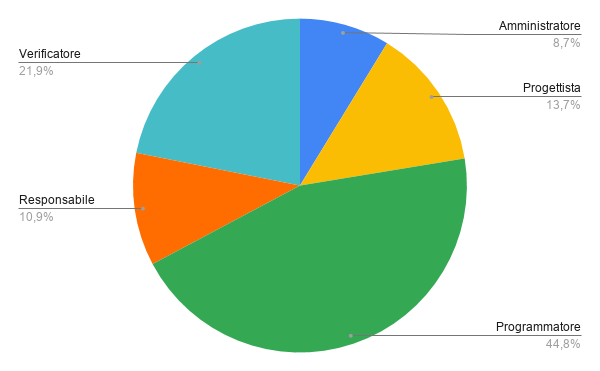
\includegraphics[width=\textwidth]{source/img/verifica_ruoli_modificato.png}
            \caption{Divisione ruoli effettiva fase di validazione e collaudo}
        \end{figure}
\subsection{Consultivo finale}
    Seguono consultivo totale, che comprende anche l'investimento iniziale, cioè l'attività che ha preceduto il colloquio RA e il consultivo totale rendicontato. Lo scopo di questa sezione è evidenziare i progressi \textit{incrementalmente} ottenuti nella pianificazione nonché le differenze di distribuzione oraria al termine dell'attività di progetto, rispetto a quanto preventivato inizialmente.
    \subsubsection{Consultivo totale}
        %startTable
        \def\salarycontent{
            {Amministratore,118,20,2360},
            {Analista,      91,25,2275},
            {Progettista,   189,22,4158},
            {Programmatore, 253,15,3795},
            {Responsabile,  67,30,2010},
            {Verificatore,  250,15,3750},
            {Totale,        968,127,18348},
        }
        %endTable
        \newcommand*\salarysummary{}
\foreach \x [count=\nj] in \salarycontent
{
    \foreach \y [count=\ni] in \x
    {
        \ifnum\ni=1
            \xappto\salarysummary{\noexpand\textbf{\y}&}
        \else\ifnum\ni=3
            \xappto\salarysummary{\noexpand\euro\ \y&}
        \else\ifnum\ni=4
            \xappto\salarysummary{\noexpand\euro\ \y}
            \gappto\salarysummary{\\}
            \gappto\salarysummary{\hline} 
        \else
            \xappto\salarysummary{\y&}
        \fi\fi\fi
    }
}

% Impostazioni della tabella
\tabulinesep = 2mm % padding
\taburowcolors [1] 2{pari .. dispari} % colori delle righe
\begin{longtabu} to \textwidth {| X[0.1, c m] | X[0.1, c m] | X[0.1, c m] | X[0.1, c m] |}
\hline
\rowcolor{header} % colore dell'header
\textbf{Ruolo} &
\textbf{Ore} &
\textbf{Costo unitario (€)} & 
\textbf{Costo totale (€)} \\
\hline
\salarysummary
\end{longtabu}
\undef\salarysummary
        La previsione iniziale era di \euro\ 17924, il motivo dell'incremento è stato riportato nella \hyperref[section:consultivo_analisi]{sezione 5.1}. In breve è stato deciso di dedicare più ore al ruolo di amministratore allo scopo di impostare al meglio l'ambiente di lavoro, questo ha portato effettivamente benefici nel lungo termine: al momento del rilascio del documento la compilazione della sorgente \LaTeX\ è completamente automatica, inoltre un sistema di notifiche avvisa i membri del team qualora ci siano problemi in fase di compilazione.
    \subsubsection{Consultivo totale rendicontato}
        %startTable
        \def\salarycontent{
            {Amministratore,54,20,1080},
            {Analista,      47,25,1175},
            {Progettista,   169,22,3718},
            {Programmatore, 253,15,3795},
            {Responsabile,  41,30,1230},
            {Verificatore,  176,15,2640},
            {Totale,        740,127,13638},
        }
        %endTable
        \newcommand*\salarysummary{}
\foreach \x [count=\nj] in \salarycontent
{
    \foreach \y [count=\ni] in \x
    {
        \ifnum\ni=1
            \xappto\salarysummary{\noexpand\textbf{\y}&}
        \else\ifnum\ni=3
            \xappto\salarysummary{\noexpand\euro\ \y&}
        \else\ifnum\ni=4
            \xappto\salarysummary{\noexpand\euro\ \y}
            \gappto\salarysummary{\\}
            \gappto\salarysummary{\hline} 
        \else
            \xappto\salarysummary{\y&}
        \fi\fi\fi
    }
}

% Impostazioni della tabella
\tabulinesep = 2mm % padding
\taburowcolors [1] 2{pari .. dispari} % colori delle righe
\begin{longtabu} to \textwidth {| X[0.1, c m] | X[0.1, c m] | X[0.1, c m] | X[0.1, c m] |}
\hline
\rowcolor{header} % colore dell'header
\textbf{Ruolo} &
\textbf{Ore} &
\textbf{Costo unitario (€)} & 
\textbf{Costo totale (€)} \\
\hline
\salarysummary
\end{longtabu}
\undef\salarysummary
        L'offerta finale ammonta a \textbf{13638 euro}. Il team si è impegnato a rimanere in linea con l'offerta finale di \textbf{13664 euro}, quando necessario, ridistribuendo l'impegno orario tra i diversi ruoli. 
\subsection{Conclusioni}
        Seguono osservazioni sull'avanzamento dell'attività di progetto e alcune considerazioni finali.
        \\ \\ \noindent
        Inizialmente la pianificazione risultava superficiale e nonostante sia stato dichiarato l'utilizzo del modello incrementale, effettivamente è stato implementato una metodologia pseudo-sequenziale. Inoltre la pianificazione era specializzata sui singoli prodotti (durante la fase di analisi solo documentali), anziché concentrarsi globalmente sull'attività di progetto. A questo è stato posto rimedio nelle fasi successive, rendendo la pianificazione più fine (e precisa). Il periodo, solitamente coincidente con l'intervallo di tempo tra una revisione di avanzamento e la successiva, è stato diviso in segmenti denominati incrementi, della durata di una settimana circa. In ogni incremento sono individuate delle attività più rilevanti, ma sempre in modo piuttosto superficiale, in modo da permettere una certa elasticità al team. Questo ha permesso un controllo più fine dell'avanzamento del progetto. Solo nell'ultima fase è stato collegato ad ogni incremento un monte ore, permettendo oltre che un consuntivo più significativo, di adeguare di incremento in incremento l'impegno orario richiesto.
        \\ \\ \noindent
        Seguono due grafici che evidenziano lo stesso trend in modi differenti: 
        \begin{itemize}
            \item il primo ci permette di individuare con più facilità le modifiche apportate ai vari ruoli;
            \item il secondo (i due grafici a torta) rende visibile la distribuzione oraria dei vari ruoli e le differenze tra il preventivato e quanto effettivamente è avvenuto.
        \end{itemize}
        \begin{figure}[H]
            \centering
            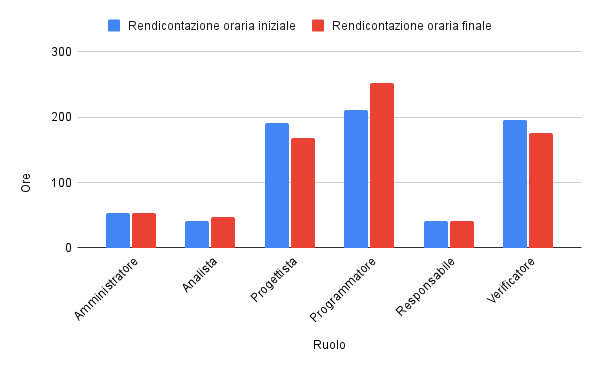
\includegraphics[width=\textwidth]{source/img/confronto_rendicontazione.png}
            \caption{Confronto rendicontazione oraria tra distribuzione preventivata contro effettiva}
        \end{figure}
        \begin{figure}[H]
            \centering
            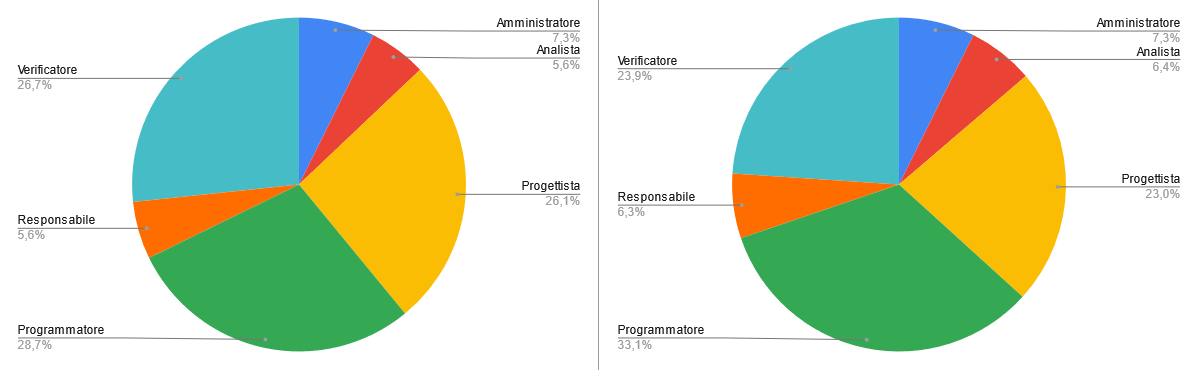
\includegraphics[width=\textwidth]{source/img/confronto_divisione_oraria.png}
            \caption{A sinistra la divisione oraria preventivata, a destra la divisione oraria finale}
        \end{figure}
        I due grafici permettono le seguenti osservazioni:
        \begin{itemize}
            \item sebbene la distribuzione oraria sia effettivamente variata, la variazione non è significativa. Ciò dimostra un buon lavoro di pianificazione dei responsabili;
            \item il \textbf{ruolo di programmatore} ha visto un incremento significativo di ore, soprattutto nell'ultima fase. Questo ruolo non era stato sottovalutato durante la pianificazione iniziale, ed era stata individuata la fase di progettazione di dettaglio e codifica come quella per cui sarebbe stato più richiesto il ruolo. Tuttavia era anche stato stimato che \hd\ e testing di quest'ultima sarebbero stati pressoché conclusi al termine della fase sopra citata. Questo non è accaduto, motivo per cui è stato richiesto un impegno importante al programmatore anche durante l'ultima fase di validazione e collaudo, per eseguire in modo soddisfacente il testing;
            \item il \textbf{ruolo di verificatore} è stato considerato subito come essenziale, si può notare come al termine dell'attività di progetto il ruolo abbia richiesto meno ore rispetto a quanto preventivato. Questo è stato possibile grazie al consolidamento del way of working per cui ogni scatto di versione richiede una verifica, e ha reso l'attività in questione molto più agevole;
            \item l'impegno orario dedicato al \textbf{ruolo di progettista} è stato invece sopravvalutato: parte della colpa va al linguaggio di programmazione richiesto, JavaScript, sebbene molto popolare, non particolarmente avanzato. Il team ha quindi deciso di utilizzare meno possibile i design pattern in quanto questi avrebbero richiesto o di utilizzare (e imparare) nuovi framework, oppure utilizzare artefici particolari per implementare costrutti non presenti nativamente nel linguaggio di programmazione utilizzato;
            \item il \textbf{ruolo di analista} ha visto un incremento delle ore a lui inizialmente dedicate: questo denota un'iniziale superficialità, durante la fase di analisi, da parte degli analisti. A questo è stato posto rimedio nelle fasi successive, il lavoro degli analisti si concretizza nel \AdR\ ritenuto ormai un documento \textit{maturo};
            \item i \textbf{ruoli di amministratore e responsabile} non hanno invece subito modifiche orarie, e i loro compiti sono rimasti i medesimi durante l'intera durata dell'attività di progetto, rispettivamente supervisione dell'ambiente di lavoro e manutenzione del documento Norme di Progetto, manutenzione del Piano di Progetto e approvazione dei documenti.
        \end{itemize}
        \noindent
        L'offerta finale ammonta a \textbf{13638 euro}, con una differenza in positivo rispetto a quanto preventivato inizialmente. Il team ritiene di aver portato a termine con successo l'attività di progetto e di aver prodotto artefatti documentali soddisfacenti e di aver raggiunto gli obiettivi richiesti dal capitolato \hd .
